\documentclass[12pt, a4paper]{article}
\usepackage{titlesec}
\usepackage{lipsum}
\usepackage{amssymb}
\usepackage{amsmath}
\usepackage[margin=1.3in]{geometry}
\usepackage[mathscr]{euscript}
\usepackage{tabto}
\usepackage{pgfplots}
\pgfplotsset{compat=1.17}

\usetikzlibrary{decorations.markings}


\DeclareSymbolFont{rsfs}{U}{rsfs}{m}{n}
\DeclareSymbolFontAlphabet{\mathscrsfs}{rsfs}
\titlelabel{\thetitle.\quad}
\righthyphenmin=1000
\lefthyphenmin=1000

\begin{document}
\section*{Unit 2}
\vspace{1em}

\subsection*{LOS 1. Solve inhomogeneous wave equation}
Problem:
\begin{gather*}
    u_{tt} - u_{xx} = f \\
    u(x, 0) = \phi(x)\\
    u_t(x,0) = \psi(x)
\end{gather*}
Solution:
\begin{gather*}
    u(x, t) = \frac{\phi(x+t) + \phi(x-t)}{2} + \frac{1}{2} \int_{[x+t, x-t]}\psi(y)dy + \frac{1}{2} \int_0^t\int_{x-(t-s)}^{x+(t-s)}f(y, s)dyds
\end{gather*}
\vspace{0.3em}

\subsection*{LOS 2. Revisit method for solving second order ODEs (homogeneous as well as inhomogeneous)}
Solve for first order homogeneous equation:
\begin{itemize}
    \item Problem statement:
    \begin{gather*}
        f: [a, b] \rightarrow \mathbb{R} \\
        f'(t) - Af(t) = 0 \\
        f(0) = v_0
    \end{gather*}
    \item Solution ($S$ is a solution operator):
    \begin{gather*}
        f(t) = e^{tA}v_0\\
        f'(t) = Ae^{tA}v_0 = Af(t)\\
        \therefore S(t)=e^tA\\
    \end{gather*}
\end{itemize}
Solve for first order inhomogeneous equation:
\begin{itemize}
    \item Problem statement:
    \begin{gather*}
        f'(t) - Af(t) = g \\
        f(0) = v_0
    \end{gather*}
    \item Solution:
    \begin{gather*}
        f(t) = \int_0^t e^{(t-s)A}g(s)ds \\
    \end{gather*}
    \item Using Liebniz integration rule to evaluate $f'(t)$:
    \begin{gather*}
        \frac{d}{dx}\left(\int_{b(x)}^{a(x)} g(s) ds\right) = g(a(x))a'(x)-g(b(x))b'(x) + \int_{b(x)}^{a(x)} \frac{\partial}{\partial x}g(s) ds\\
        \frac{d}{dx}\left(\int_0^t e^{(t-s)A}g(s)ds\right) = g(t) + \int_{b(x)}^{a(x)} \frac{\partial}{\partial t}e^{(t-s)A}g(s) ds\\
        \frac{d}{dx}\left(\int_0^t e^{(t-s)A}g(s)ds\right) = g(t) + A\int_{b(x)}^{a(x)}e^{(t-s)A}g(s) ds\\
        \frac{d}{dx}\left(\int_0^t e^{(t-s)A}g(s)ds\right) = g(t) + Af(t)\\
        f'(t) = g(t) + Af(t)\\
    \end{gather*}
\end{itemize}
Solve for second order differential equation:
\begin{itemize}
    \item Problem statement:
    \begin{gather*}
        f''(t) - Af(t) = 0 \\
        f(0) = v_0
    \end{gather*}
    \item Assume solution takes the form $e^{i\xi t}$:
    \begin{gather*}
        f(t) = e^{i\xi t} \\
        f''(t) = \xi^2e^{i\xi t} = Af(t) \\
        -\xi^2e^{i\xi t} = Ae^{i\xi t} \\
        \therefore \xi = \pm i \sqrt{A}
    \end{gather*}
    \item Solutions:
    \begin{gather*}
        f(t) = e^{i\sqrt{A}t} \qquad\qquad f(t) = e^{-i\sqrt{A}t} \\
        S_+(t) = e^{i\sqrt{A}t} \qquad\qquad S_-(t) = e^{-i\sqrt{A}t} \\
        S(t) = C_1e^{i\sqrt{A}t} + C_2e^{-i\sqrt{A}t}
    \end{gather*}
    \item In Dirichlet problem:
    \begin{gather*}
        f''(t) - Af(t) = 0 \\
        f(0) = v_0\\
        f'(0) = 0
    \end{gather*}
    \begin{gather*}
        S_D(t) = f(t) = C_1e^{i\sqrt{A}t} + C_2e^{-i\sqrt{A}t} \\
        f(t) = C_1(cos\sqrt{A}t + isin\sqrt{A}t) + C_2(cos\sqrt{A}t - isin\sqrt{A}t) \\
        f(t) = (C_1 + C_2)(cos\sqrt{A}t) + i(C_1-C_2)(sin\sqrt{A}t) \\
        f(0) = (C_1 + C_2)(1) + 0 = v_0\\
        (C_1 + C_2)= v_0 
    \end{gather*}
    \begin{gather*}
        \dot{S}_D(t) = f'(t) = v_0\sqrt{a}(sin\sqrt{A}t) + i(C_1-C_2)\sqrt{A}(sin\sqrt{A}t) \\
        f'(0) = 0 + i(C_1-C_2)\sqrt{A} =0 \\
        (C_1-C_2) = 0
    \end{gather*}
    \begin{gather*}
        \therefore f(t) = v_0cos\sqrt{a}t \rightarrow S_D(t) = cos\sqrt{a}t
    \end{gather*}
    \item In Neumann problem:
    \begin{gather*}
        f''(t) - Af(t) = 0 \\
        f(0) = 0\\
        f'(0) = v_1
    \end{gather*}
    \begin{gather*}
        S_N(t) = (C_1 + C_2)(cos\sqrt{A}t) + i(C_1-C_2)(sin\sqrt{A}t) \\
        f(0) = (C_1 + C_2)(1) + 0 = 0\\
        (C_1 + C_2)= 0
    \end{gather*}
    \begin{gather*}
        \dot{S}_N(t)=f'(t) = i(C_1-C_2)\sqrt{A}(sin\sqrt{A}t) \\
        f'(0) = 0 + i(C_1-C_2)\sqrt{A} =v_1 \\
        (C_1-C_2) = \frac{v_1}{\sqrt{A}}
    \end{gather*}
    \begin{gather*}
        \therefore f(t) = \frac{v_1sin\sqrt{A}t}{\sqrt{A}} \rightarrow S_N(t) = \frac{sin\sqrt{A}t}{\sqrt{A}}
    \end{gather*}
    \item Solution for inhomogeneous problem:
    \begin{gather*}
        f''(t) - Af(t) = g(t) \\
        f(0) = v_0 \\
        f'(0) = v_1 \\
        f(t) = S_D(t)v_0 + S_N(t)v_1 + \int_0^tS_N(t-s)g(s)ds 
    \end{gather*}

\end{itemize}

\vspace{0.3em}
    
\subsection*{LOS 3. Solve inhomogeneous wave equation using Green’s formula and the operator method}
Solving using Green's formula:
\begin{itemize}
    \item Evaluate integral of the original equations:
    \begin{gather*}
        u_{tt} - c^2u_{xx} = f(x, t) \\
        \iint_{\Delta}(u_{tt} - c^2u_{xx}) = \iint_{\Delta}f
    \end{gather*}
    \item Green's theorem:
    \begin{gather*}
        \iint_{\Delta}(P_x - Q_t)dxdt = \oint_{\Delta}(Pdt + Qdx) \\
        \iint_{\Delta}(- c^2u_{xx}-u_{tt}) = \int_{L_0+L_1+L_2} (-c^2u_xdt + u_tdx)
    \end{gather*}
\end{itemize}
Example, wave equation without reflection:\\
\begin{center}
    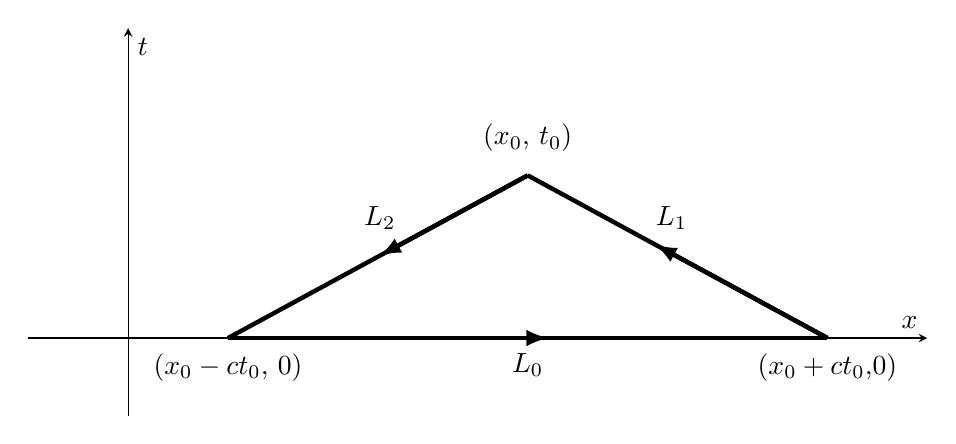
\begin{tikzpicture}
        \begin{axis}[
            ticks=none,
            xmin=-0.25, xmax=2,
            ymin=-0.25, ymax=1,
            every axis x label/.style={
                at={(ticklabel* cs:1.0)},
                anchor=west,
            },
            every axis y label/.style={
                at={(ticklabel* cs:1.0)},
                anchor=south,
            },
            xlabel={$x$},
            ylabel={$t$},
            axis lines=center,
            axis on top=true,
            width=13cm,
            height=6.5cm,
            ]
            \addplot[-latex] [mark=none,domain=0.25:1.05,draw=black,ultra thick, postaction={decorate}] {0};
            \addplot[latex-] [mark=none,domain=0.63:1.0,draw=black,ultra thick] {0.7*(x-0.25)};
            \addplot[latex-] [mark=none,domain=1.32:1.75,draw=black,ultra thick] {-0.7*(x-1.75)};
            \addplot [mark=none,domain=0.25:1.75,draw=black,ultra thick, postaction={decorate}] {0};
            \addplot [mark=none,domain=0.25:1,draw=black,ultra thick] {0.7*(x-0.25)};
            \addplot [mark=none,domain=1:1.75,draw=black,ultra thick] {-0.7*(x-1.75)};
            \node[label=below:{($x_0-ct_0$, 0)},inner sep=2pt] at (axis cs:0.25,0){};
            \node[label=below:{($x_0+ct_0$,0)},inner sep=2pt] at (axis cs:1.75,0){};
            \node[label=above:{($x_0$, $t_0$)},inner sep=2pt] at (axis cs:1,0.55){};
            \node[label=below:{$L_0$},inner sep=2pt] at (axis cs:1,0){};
            \node[label=above:{$L_2$},inner sep=2pt] at (axis cs:0.63,0.3){};
            \node[label=above:{$L_1$},inner sep=2pt] at (axis cs:1.36,0.3){};
        \end{axis}
    \end{tikzpicture}
\end{center}
\begin{itemize}
    \item On $L_0$:
    \begin{gather*}
        t = 0 \\
        dt = 0 \\
        u_t(x, 0) = \psi(x) \\
        \therefore \int_{L_0} = \int_{L_0} (0 - u_t(x, 0) dx) = -\int_{x_0-ct_0}^{x_0+ct_0}\psi(x)dx
    \end{gather*}
    \item On $L_1$:
    \begin{gather*}
        x + ct = x_0 + ct_0  \\
        dx + cdt = 0 \rightarrow dt = \frac{-dx}{c}, dx = -cdt\\
        -c^2u_xdt - u_tdx =  cu_xdx + cu_tdt = cdu\\
        \therefore \int_{L_1} = c\int_{L_1} du = c(u(x_0, t_0) - u(x_0+ct_0, 0)) = cu(x_0, t_0) - c\phi(x_0 +ct_0)
    \end{gather*}
    \item On $L_2$:
    \begin{gather*}
        x - ct = x_0 - ct_0  \\
        dx - cdt = 0 \rightarrow dt = \frac{dx}{c}, dx = cdt\\
        -c^2u_xdt - u_tdx =  -cu_xdx - cu_tdt = -cdu\\
        \therefore \int_{L_2} = -c\int_{L_2} du = -c(u(x_0-ct_0, 0) - u(x_0, t_0)) = -c\phi(x_0 -ct_0) +cu(x_0, t_0)
    \end{gather*}
    \item Solution:
    \begin{gather*}
        \iint_{\Delta}f = -\int_{x_0-ct_0}^{x_0+ct_0}\psi(x)dx + 2cu(x_0, t_0) - c\phi(x_0 +ct_0) -c\phi(x_0 -ct_0)\\
        u(x_0, t_0) = \frac{1}{2c}\iint_{\Delta}f  + \frac{1}{2}[\phi(x_0 +ct_0) -\phi(x_0 -ct_0)] -\frac{1}{2c}\int_{x_0-ct_0}^{x_0+ct_0}\psi(x)dx \\
    \end{gather*}
\end{itemize}
Solving using operator method:
\begin{itemize}
    \item By ODE analogy, solution takes the following form:
    \begin{gather*}
        u(t) = S_D(t)v_0 + S_N(t)v_1 + \int_0^tS_N(t-s)f(s)ds 
    \end{gather*}
    \item Define source operator, $\mathscrsfs{L}$ such that it solve the Neumann problem:
    \begin{gather*}
        u_{tt} - u_{xx} = f \qquad u(x, 0) = 0\qquad u_t(x,0) = \psi(x) \\
        \mathscrsfs{L}(t)\psi= \frac{1}{2c}\int_{x-ct}^{x+ct}\psi(y)dy
    \end{gather*}
    \item Solution for Dirichlet problem:
    \begin{gather*}
        u_{tt} - u_{xx} = f \qquad u(x, 0) = \phi(x)\qquad u_t(x,0) = 0 \\
        \frac{\partial}{\partial t}\mathscrsfs{L}(t)\phi= \frac{\partial}{\partial t}\frac{1}{2c}\int_{x-ct}^{x+ct}\phi(y)dy = \frac{1}{2}[\phi(x +ct) -\phi(x -ct)]
    \end{gather*}
    \item Solution for inhomogeneous problem:
    \begin{gather*}
        u_{tt} - u_{xx} = f \qquad u(x, 0) = 0\qquad u_t(x,0) = 0 \\
        u(t)= \int_0^t \left[\frac{1}{2c}\int_{x-(t-s)}^{x+(t-s)}f(y, s)dy\right]ds = \frac{1}{2c}\iint_{\Delta}fdxdt
    \end{gather*}
\end{itemize}

\vspace{0.3em}

\subsection*{LOS 4. Learn the Duhamel principle}
Using Duhamel's principle we can get the following solution to the wave equation:
\begin{gather*}
    u_{tt} - c^2u_{xx} = f(x,t) \\
    u(x, 0) = \phi(x)\\
    u_t(x,0) = \psi(x)
\end{gather*}
\begin{gather*}
    u(x, t) = \frac{\phi(x+ct) + \phi(x-ct)}{2} + \frac{1}{2c} \int_{x-ct}^{x+ct}\psi(y)dy + \frac{1}{2c} \int_0^t\int_{x-c(t-s)}^{x+c(t-s)}f(y, s)dyds\\
\end{gather*}
Duhamel's principle states that if you can solve the homogeneous equation, you can also solve the inhomogeneous equation:
\begin{itemize}
    \item Given the following problem:
    \begin{gather*}
        u_{tt} - c^2u_{xx} = f(x,t) \\
        u(x, 0) = \phi(x)\\
        u_t(x,0) = \psi(x)
    \end{gather*}
    \item We can solve the following problem to get the inhomogeneous solution:
    \begin{gather*}
        u_{tt} - c^2u_{xx} = f(x,t) \\
        u(x, 0) = 0\\
        u_t(x,0) = f(x, t)dt
    \end{gather*}
    \item Where the solution is as follow:
    \begin{gather*}
        u(x, t) = \int \frac{\partial}{\partial t} f(x, t)dt
    \end{gather*}
\end{itemize}





\vspace{0.3em}

\subsection*{LOS 5. Study well-poseness of wave equation}
Conditions for well-poseness:
\begin{enumerate}
    \item Existence: solution has an explicit formula
    \item Uniqueness: solution using different methods are the same
    \item Stability: use norms\\
\end{enumerate}
Wave equation norms:
\begin{enumerate}
    \item $|u_D(x, t)| \leq \|\phi\|_\infty$ for all $x$, $t$ \\
    $\rightarrow \sup_x|u_D(x, t)| \leq \|\phi\|_\infty$\\
    \item $|u_N(x, t)| = |\frac{1}{2}\int_{x-ct}^{x+ct}\psi(y)dy| \leq \frac{1}{2}\int_{x-ct}^{x+ct}|\psi(y)|dy \leq t\|\psi\|_\infty$ \\ $\rightarrow \sup_x|u_N(x, t)| \leq t\|\psi\|_\infty$\\
    $\rightarrow\sup_{x, t}|u_N(x, t)| \leq \frac{\|\psi\|_1}{2}$\\
    \item $|u_{source}(x, t)| \leq \frac{1}{2}\int_{x-(t-s)}^{x+(t-s)}dsdy \|g\|_\infty \\= \int_0^t(t-sds)\|g\|_\infty = \int_0^tsds\|g\|_\infty \leq \frac{t^2}{2}\|g\|_\infty$ \\
    $\rightarrow |u_{source}(x, t)| \leq \frac{t^2}{2}\|g\|_\infty$
\end{enumerate}
\vspace{0.3em}

\subsection*{LOS 6. Learn how to calculate different norms}
Norms:
\begin{enumerate}
    \item p-norm:
    \begin{gather*}
        \|\phi\|_P = \left(\int_{\mathbb{R}}|\phi(x)|^Pdx\right)^{\frac{1}{P}}
    \end{gather*}
    \item infinity-norm/sup-norm/uniform-norm:
    \begin{gather*}
        \|\phi\|_{\infty}  = \sup_x|\phi(x)|\\
        \|\phi\| = \max_{x}|\phi(x)|\\
        \|\phi\|_T = \max_{x, 0\leq t\leq T}|\phi(x, t)|
    \end{gather*}
    {\tiny*($\sup$ refers to the smallest upper bound of the set)}
    \item 1-norm:
    \begin{gather*}
        \|\phi\|_1 = \int_{\mathbb{R}}|\phi(x)|dx
    \end{gather*}
    \item $l^2$-norm:
    \begin{gather*}
        \|\phi\|^2 = \int_{\mathbb{R}}|\phi(x)|^2dx\\
        \|\phi\| = \sqrt{\int_{\mathbb{R}}|\phi(x)|^2dx}
    \end{gather*}
\end{enumerate}
\vspace{0.3em}

\subsection*{LOS 7. Study reflection of waves}
Lemma:
\begin{enumerate}
    \item $\phi$ odd $\implies u_D$ odd, $\phi$ even $\implies u_D$ even
    \item $\psi$ odd $\implies u_N$ odd, $\psi$ even $\implies u_N$ even \\
\end{enumerate}
Wave-equation homogeneous problem on the half-line:
\begin{itemize}
    \item Problem:
    \begin{gather*}
        u_{tt} - u_{xx} = 0 \qquad\text{for }0<x<\infty\\
        u(x, 0) = \phi(x)\\
        u_t(x,0) = \psi(x)\\
        u(0, t)=0
    \end{gather*}
    \item Use odd extension:
    \[ \phi_{odd}(x) = \begin{cases} 
        \phi(x) & x > 0 \\
        -\phi(-x) & x > 0 \\
        0 & x = 0
     \end{cases}
    \]
    \[ \psi_{odd}(x) = \begin{cases} 
        \psi(x) & x > 0 \\
        -\psi(-x) & x > 0 \\
        0 & x = 0
     \end{cases}
    \]
    \item Solution:
    \begin{gather*}
        u(x, t) = \frac{\phi_{odd}(x+ct) + \phi_{odd}(x-ct)}{2} + \frac{1}{2c} \int_{x-ct}^{x+ct}\psi_{odd}(y)dy \\
        u(x, t) = \frac{\phi(x+ct) + \phi(x-ct)}{2} + \frac{1}{2c} \int_{x-ct}^{x+ct}\psi(y)dy \qquad \text{if } x > c|t|\\
        u(x, t) = \frac{\phi(ct+x) - \phi(ct-x)}{2} + \frac{1}{2c} \int_{ct-x}^{ct+x}\psi(y)dy \qquad \text{if } x < c|t|\\
    \end{gather*}
\end{itemize}
Wave-equation inhomogeneous problem on the half-line:
\begin{itemize}
    \item Problem:
    \begin{gather*}
        u_{tt} - u_{xx} = f(x, t) \qquad\text{for }0<x<\infty\\
        u(x, 0) = \phi(x)\\
        u_t(x,0) = \psi(x)\\
        u(0, t)= h(t)
    \end{gather*}
    \item Solution (reflected once):
    \begin{gather*}
        u(x, t) = u_D(x, t) + u_N(x, t) + h(t-\frac{x}{c})+\frac{1}{2} \int_0^t\int_{x-(t-s)}^{x+(t-s)}f(y, s)dyds
    \end{gather*}
\end{itemize}
\vspace{0.3em}

\subsection*{LOS 8. Find the periodic solutions for the wave equation}
Wave-equation homogeneous problem on the finite interval:
\begin{itemize}
    \item Problem:
    \begin{gather*}
        u_{tt} - u_{xx} = f(x, t) \qquad\text{for }0<x<l\\
        u(x, 0) = \phi(x)\\
        u_t(x,0) = \psi(x)\\
        u(0, t)=h(t)
    \end{gather*}
    \item Use periodic extension:
    \[ \phi_{ext}(x) = \begin{cases} 
        \phi(x) & x > 0 \\
        -\phi(-x) & x > 0 \\
        \text{extended to be of period 2l}
     \end{cases}
    \]
    \[ \psi_{odd}(x) = \begin{cases} 
        \psi(x) & x > 0 \\
        -\psi(-x) & x > 0 \\
        \text{extended to be of period 2l}
     \end{cases}
    \]
    \item Solution:
    \begin{gather*}
        u(x, t) = \frac{\phi_{ext}(x+ct) + \phi_{ext}(x-ct)}{2} + \frac{1}{2c} \int_{x-ct}^{x+ct}\psi_{ext}(y)dy \\
    \end{gather*}
\end{itemize}
Wave-equation inhomogeneous problem on the half-line:
\begin{itemize}
    \item Problem:
    \begin{gather*}
        u_{tt} - u_{xx} = f(x, t) \qquad\text{for }0<x<l\\
        u(x, 0) = \phi(x) \rightarrow 0\\
        u_t(x,0) = \psi(x)\rightarrow 0\\
        u(0, t)= h(t) \qquad u(l, t) = k(t)
    \end{gather*}
    \item Solution:
    \begin{gather*}
        u(x, t) = \sum_{n=0}^{O_{odd}-1}h\left(t-\frac{x}{c}-\frac{2nl}{c}\right) - \sum_{n=0}^{O_{even}-1}h\left(t-\frac{l-x}{c}-\frac{(2n+1)l}{c}\right) \\- \sum_{n=0}^{L_{odd}-1}k\left(t-\frac{x}{c}-\frac{(2n+1)l}{c}\right) + \sum_{n=0}^{L_{even}-1}k\left(t-\frac{l-x}{c}-\frac{2nl}{c}\right)
    \end{gather*}

    \begin{enumerate}
        \item $O_{odd}$: number of odd reflections at $x=0$
        \item $O_{even}$: number of even reflections at $x=0$
        \item $L_{odd}$: number of odd reflections at $x=l$
        \item $L_{even}$: number of even reflections at $x=l$
    \end{enumerate}
\end{itemize}
\vspace{0.3em}
\vspace{0.3em}

\subsection*{LOS 9. Learn inner product spaces and its properties}
Define $v$ as a vector in $\mathbb{C}$ such that:
\begin{enumerate}
    \item $(v+w) + z = v+(w+z)$
    \item $\lambda(v+w) = \lambda v + \lambda w$
    \item $(v, w+\lambda z) = (v, w) + \lambda (v, z)$
    \item $\overline{(v, w)} = (w, v)$, $b = \alpha + i\beta \rightarrow \bar{b} = \alpha - i\beta$
    \item $(v, v)\geq 0$
    \item $(v, v) = 0 \Longleftrightarrow v=0$\\
\end{enumerate}
Inner product definitions:
\begin{itemize}
    \item For $v = \mathbb{C}$:
    \begin{gather*}
        (v, v) = \bar{v}v \geq 0
    \end{gather*}
    \item For $v = \mathbb{C}^n$:
    \begin{gather*}
        (v, w) = \sum_{j=1}^n\bar{v_j}w_j\\
        (v, v) = \sum_{j=1}^n|v_j| = \|v\|^2
    \end{gather*}
    \item For $v = \mathbb{R}^n$:
    \begin{gather*}
        (v, w) = \sum v_jw_j\\
        (v, v) = v\cdot v \geq 0
    \end{gather*}
\end{itemize}
Examples:
\begin{itemize}
    \item For $v=C[0,1]$:
    \begin{gather*}
        (f+\lambda g)(t) = f(t) + \lambda g(t) \\
        (f, g) = \int_0^1\overline{f(t)}g(t)dt
    \end{gather*}
    \item For $v=C[0,2\pi]$:
    \begin{gather*}
        (f, g) = \int_0^{2\pi}\overline{f(t)}g(t)\frac{dt}{2\pi}\\
    \end{gather*}
\end{itemize}
Cauchy-Swarsch:
\begin{itemize}
    \item $\|v\| = (v, v)^{\frac{1}{2}}$
    \item $\|v+w\| \leq \|v\| + \|w\|$
    \item $v \perp w$ if $(v, w) = 0 \Leftrightarrow \|v+w\| = \|v\| + \|w\|$
    \item $|(v, w)| \leq \|v\|\|w\|$
\end{itemize}
\vspace{0.3em}

\subsection*{LOS 10. Understand the orthogonal and orthonormal families of functions}
Orthogonal and orthonormal family:
\begin{enumerate}
    \item Orthogonal $\Leftrightarrow (v_j, v_{j'}) = 0\quad\forall j \ne j'$
    \item Orthonormal $\Leftrightarrow (v_j, v_{j'}) = 0\quad\forall j \ne j'$ and $(v_j, v_{j'}) = 1\quad\forall j = j'$ \\
\end{enumerate}
Let $(v_j)\;\forall j$ be an orthogonal family:
\begin{gather*}
    \left\|\sum \lambda_jv_j\right\|^2 = \sum_j|\lambda_j|^2
\end{gather*}
Proposition:
\begin{itemize}
    \item Let $(v_j)^n_{j=1}$ be orthonormal.
    \item Let $W = \{\sum_{j=1}^n\lambda_jv_j \; : \; \lambda_j \in \mathbb{C}\}$.
    \item Let $x\notin W$. Define $P(x) = \sum_{j=1}^{n}(v_j, x)v_j$
    \item Then $\inf \|x-y\| = \|x-P_x\|, y \in W$
\end{itemize}
\vspace{0.3em}

\end{document}